\chapter{Mercoledì 06/05/2020}
\section{Gestione delle transazioni}
Noi abbiamo sistemi di tabelle che contengono informazioni diverse: gestione impianti, immissione di ordini di servizio, amministrazione, gestione elenchi abbonati... In alcune circostanze queste tabelle necessitano di essere visualizzate insieme.
\begin{center}
	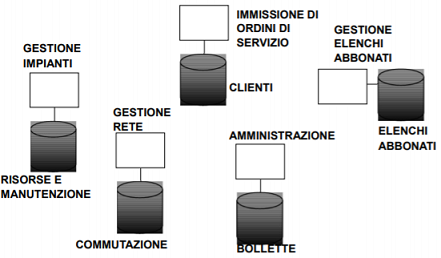
\includegraphics{images/131.PNG}
\end{center}
Dobbiamo tenere conto, come al solito, delle connessioni simultanee da parte di più utenti in uno stesso momento.  Solitamente un DBMS è multiutente, cioè può essere usato contemporaneamente da più utenti.
\paragraph{Modalità interleaved o concorrente}  I sistemi utilizzati molti anni fa, con una sola CPU, erano già in grado di gestire un utilizzo concorrente del sistema. Un sistema solitamente è di tipo multitasking, cioè permette l'esecuzione in simultanea di più operazioni. Se si ha una sola CPU in realtà si può eseguire una sola operazione: semplicemente ci si limita ad eseguire un'operazione, a sospenderla temporaneamente per portarne avanti un'altra, e così via.
Un'esecuzione dei processi può risultare, pertanto, concorrente o alternata (\emph{interleaved}).
\paragraph{Definizione di transazione} Le transazione non è un'operazione ma un insieme di comandi base: un'unità elementare di lavoro. A questa sequenza voglio associare caratteristiche quali la robustezza, la correttezza e l'isolamento (cioè non posso vedere l'interno della transazione e l'esito fino a conclusione). La cosa può essere immaginata anche nell'ambito MySQL con inserimenti, cancellazioni, modifiche o interrogazioni. I sistemi attualmente utilizzati sono transazionali: eseguono transazioni per conto di un certo numero di applicazioni concorrenti.
\pagebreak
Una transazione coinvolge generalmente più tabelle con le sue operazioni:
\begin{center}
	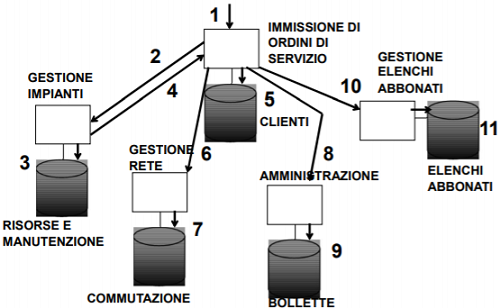
\includegraphics{images/132.PNG}
\end{center}
Si inizia e si termina con i seguenti comandi, rispettivamente
\begin{verbatim}
	begin transaction
	end transaction
\end{verbatim}
Uno dei due comandi deve essere eseguito una e una sola volta all'interno della transazione:
\begin{verbatim}
	commit work
	rollback work
\end{verbatim}
Col primo eseguiamo la transazione con tutti i suoi comandi, col secondo blocchiamo tutto e non eseguiamo niente (è come se non avessi eseguito nessuna delle operazioni presenti nella transazione).

\paragraph{Proprietà delle transazioni ($ACID$)}
\begin{itemize}
	\item \textbf{Atomicità}. Gli stati intermedi della transazione non si vedono: vedono lo stato iniziale corretto e lo stato finale, che dipendono dal comando eseguito (commit o rollback). Nel caso di errore dobbiamo:
	\begin{itemize}
		\item annullare le operazioni svolte se ci troviamo prima del commit
		\item ripetere le operazioni già fatte se ci troviamo dopo il commit
	\end{itemize}
	Normalmente l'esito è il commit. L'abort può essere richiesto dall'applicazione (suicidio) o dal sistema (omicidio)
	\item \textbf{Consistenza}. Devono essere rispettati i vincoli di integrità: ciò avviene se sono corretti lo stato iniziale e quello finale. Nel corso della transazione posso avere incosistenze, l'importante è che non ci siano alla fine.
	\item \textbf{Isolamento}. Gli stati intermedi non vengono resi visibili agli altri processi. L'esecuzione concorrente di più transazioni deve produrre un risultato ottenibile mediante esecuzione sequenziale.
	\item \textbf{Durata}. Quanto fatto da una transazione andata in commit non viene perso. I guasti non hanno effetto sul sistema poichè si interviene per recuperare uno stato consistente.
\end{itemize}

\paragraph{Stati di una transazione}
\begin{itemize}
	\item \textbf{active}. Dopo il begin-transaction posso eseguire operazioni di lettura e scrittura.
	\item \textbf{partially committed}. Lo stato viene raggiunto dopo averr eseguito l'ultima operazione. Il gestore dell'affidabilità si assicura che le operazioni possano essere eseguite senza problemi
	\item \textbf{committed}. Si passa a questo stato se i controlli precedenti danno esito positivo.
	\item \textbf{failed}. Lo stato viene raggiunto se la verifica precedente fallisce
	\item \textbf{aborted}. Si ha un rollback: la base di dati mantiene consistenza e le operazioni non vengono eseguite.
\end{itemize}
\paragraph{Gestori}
L'atomicità e la durabilità sono garantiti dal \emph{gestore dell'affidabilità}, l'isolamento dal \emph{gestore della concorrenza}, la consistenza dal \emph{gestore dell'integrità a tempo di esecuzione}.
\begin{center}
	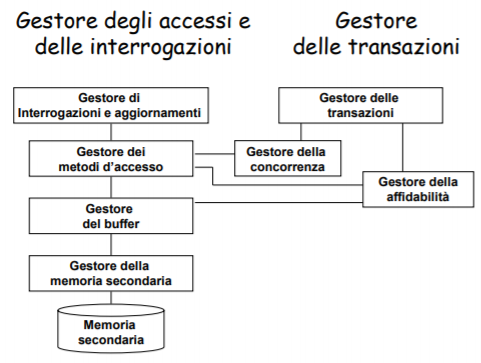
\includegraphics{images/133.PNG}
\end{center}
\paragraph{Gerarchia di memoria} All'interno della memoria distinguiamo due aree di memoria:
\begin{itemize}
	\item la \textbf{memoria principale}, volatile. I dati vengono persi quando si spenge il dispositivo
	\item la \textbf{memoria secondaria}, permanente. I dati permangono rispettando una delle proprietà tipiche della base di dati (la persistenza). In questa area si troverà la base di dati vera e propria, che deve sopravvivere alle esecuzioni dei programmi.
\end{itemize}
Queste sono organizzate in modo diverso: la memoria secondaria è organizzata in blocchi di lunghezza generalmente fissa. Le uniche operazioni possibili sono lettura e scrittura dei dati di un blocco. La memoria principale, invece, è organizzata in pagine. 
\paragraph{Buffer} Il buffer (struttura fisica) permette l'interfacciamento del database, presente in memoria secondaria, con la memoria principale. Si trova anch'esso nella memoria principale ed è un elemento intermedio: ciò che deve essere letto dal computer viene spostato dalla memoria secondaria al buffer. Segue un numero di accessi estremamente limitato alla memoria secondaria (operazione più costosa).
\begin{itemize}
	\item Il buffer è gestito dal DBMS
	\item Risulta organizzato in pagine (come già detto si trova in memoria principale)
	\item Considerando l'equivalenza pagina-blocco il caricamento di una pagina del buffer richiede una lettura in memoria secondaria, mentre il salvataggio richiede un'operazione di scrittura.
\end{itemize}
Il gestore del buffer:
\begin{itemize}
	\item riceve richieste di lettura e scrittura di pagine dalle transazioni
	\item le esegue accedendo alla memoria secondaria solo quando indispensabile
	\item le pagine vengono mantenute finchè il buffer non è pieno e non possono essere inserite altre pagine
\end{itemize}
\paragraph{Località dei dati} La probabilità di dover riutilizzare i dati attualmente in uso è molto alta. La \emph{legge di Pareto} afferma che l'80\% delle operazioni utilizza sempre lo stesso 20\% dei dati!
\paragraph{Primitive di interfacciamento} Il buffer funge da interfaccia ed esegue una serie di primitive.
\begin{itemize}
	\item \textbf{fix}. Richiesta di una pagina, lettura solo se la pagina non è nel buffer
	\item \textbf{setDirty}. Comunica che la pagina è stata modificata
	\item \textbf{unfix}. Comunica che la transazione ha concluso l'utilizzo della pagina (e quindi la stessa può essere richiesta da altre transazioni).
	\item \textbf{Force}. Trasferisce una pagina nella memoria secondaria su richiesta del \emph{gestore dell'affidabilità}.
\end{itemize}

\section{Gestione dell'affidabilità}
Il gestore dell'affidabilità viene messo in funzione in presenza di malfunzionamenti, solitamente dovuti a
\begin{itemize}
	\item \textbf{errori software} che portano a risultati scorretti
	\item \textbf{malfunzionamenti fisici}, come per esempio la mancanza di corrente in assenza di un generatore o un errore durante il trasferimento di dati (malfunzionamento del disco). I dati presenti nella memoria principale non sono più affidabili, quelli nella memoria secondaria sì.
\end{itemize}
Dobbiamo tener conto che i risultati intermedi sono salvati nel buffer, appartenente alla memoria principale. Se viene meno l'alimentazione i dati del buffer saranno persi (segue una certa procedura di recupero). In altre circostanze potrei avere anche errori legati alla memoria secondaria!
\begin{center}
	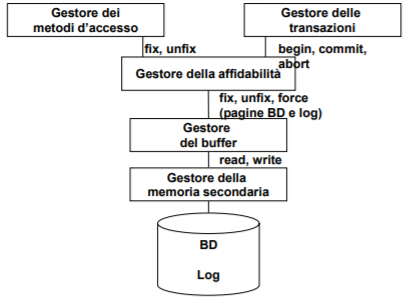
\includegraphics{images/134.PNG}
\end{center}
\begin{itemize}
	\item \underline{Garantisce atomicità e durabilità}.
	\item Prende in considerazione il begin/commit/abort
	\item Collabora col gestore del buffer in modo che le informazioni vengano poste in memoria secondaria.
	\item Si garantisce che l'esecuzione dei comandi transazionali e le operazioni di ripristino siano sempre eseguite garantendo la consistenza della base di dati
	\item Archivia le operazioni svolte in log (strumento necessario per fare quanto detto prima): esso consiste in un file sequenziale gestito dal controllore e scritto in memoria stabile. Le operazioni sono riportate in ordine e se ne hanno più copie in modo da non perderli in caso di disastri naturali.
\end{itemize}
\paragraph{Tipi di memoria} Le memorie, ai fini del ripristino, vengono classificate in volatili, non volatili e stabili. 
\paragraph{Memoria stabile} La memoria stabile ospita i log. Non può danneggiarsi e non esiste in natura (astrazione). La sua ``esistenza'' è perseguita attraverso le ridondanze (un numero elevatissimo di copie tra vari dischi e oggetti).
\paragraph{Log} Il log è un file sequenziale, gestito dal controllore dell'affidabilità e posto in memoria stabile. Può essere immaginato come un diario di bordo: in esso vengono salvate le operazioni delle transazioni e i record di sistema
\begin{itemize}
	\item \textbf{Operazioni delle transazioni} (attività svolte dalle transazioni):
	\begin{itemize}
		\item begin $B(T)$
		\item insert $I(T,O,AS)$
		\item delete $D(T,O,BS)$
		\item update $U(T,O,BS,AS)$
		\item commit $C(T)$
		\item abort $A(T)$
	\end{itemize}
	dove $T$ è l'identificativo della transazione, $BS$ lo stato prima della modifica, $AS$ lo stato dopo la modifica, $O$ l'oggetto coinvolto nell'operazione.
	\item \textbf{Record di sistema} (scritti dal controllore dell'affidabilità):
	\begin{itemize}
		\item dump
		\item checkpoint
	\end{itemize}
\end{itemize}
\paragraph{Struttura del log}
\begin{center}
	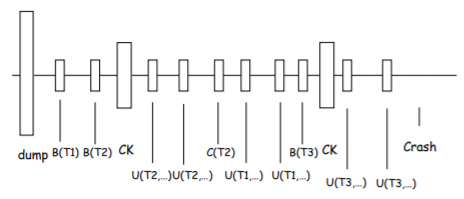
\includegraphics{images/135.PNG}
\end{center}
\begin{itemize}
	\item \textbf{dump}: copia di un database in un certo momento (supponiamo, per esempio, che venga fatta una copia ogni 12 ore).
	\item \textbf{checkpoint}: visione dello stato delle transazioni. Permette una ricostruzione più agevole delle operazioni eseguite in modo da evitare, in caso di errori, una ripartenza da zero.
\end{itemize}
\paragraph{Operazione Checkpoint} Operazione che ha lo scopo di registrare quali transazioni sono attive in un certo istante, cioè le transazioni \emph{a metà strada}. In contemporanea vogliamo essere certi che le altre operazioni non siano iniziate o siano finite. Cosa faccio ogni volta che eseguo questa operazione?
\begin{itemize}
	\item Sospendo l'accettazione di operazioni di commit/abort
	\item Si forza la scrittura in memoria di massa delle pagine di buffer modificate da transazioni in commit
	\item Si forza la scrittura nel log di record
	\item Si riprende ad accettare tutte le operazioni
\end{itemize}
Tutto questo permette di garantire la persistenza delle transazioni che hanno eseguito il commit.
\paragraph{Dump} Il dump consiste in una copia completa della base di dati. Solitamente viene prodotta mentre il sistema non è operativo e salvata in memoria stabile come backup.
\paragraph{Operazioni di undo e redo}
\begin{itemize}
	\item Undo di una azione su un oggetto $O$:
	\begin{itemize}
		\item update, delete: copiare il valore del before state nell'oggetto $O$
		\item insert: eliminare $O$
	\end{itemize}
	\item Redo di una azione su un oggetto $O$:
	\begin{itemize}
		\item insert,update: copiare il valore dell'after state nell'oggetto $O$
		\item delete: eliminare $O$
	\end{itemize}
\end{itemize}
\paragraph{Idempotenza di undo e redo} Posso compiere le operazioni più volte, il risultato rimane sempre lo stesso:
\begin{itemize}
	\item $undo(undo(A))=undo(A)$
	\item $redo(redo(A))=redo(A)$
\end{itemize}
\paragraph{Quando il controllore dell'affidabilità può consentire la modifica del log da parte delle transazioni}
Possiamo usare una delle seguenti regole:
\begin{itemize}
	\item \textbf{Regola Write-Ahead-Log}: letteralmente \emph{scrivi il log per primo}, impongo che il $BS$ dei record del log venga scritto prima di effettuare la corrispondente operazione sul database. 
	\item \textbf{Regola Commit-Precedenza}: si scrive la parte $AS$ dei record di log prima di effettuare il commit.
\end{itemize}
Nella pratica entrambe le componenti vengono scritte nel record in contemporanea. In modo semplificato possiamo dire:
\begin{itemize}
	\item \textbf{Regola W-A-L}: scrivere i record di log prima delle corrispondenti operazioni nella base di dati (dopo il commit)
	\item \textbf{Regola C-P}: scrivere i record di log prima dell'operazione di commit
\end{itemize}
\paragraph{Esito di una transazione} L'esito di una transazione è determinato in modo irrevocabile quando si scrive il record di commit del log. Segue un comportamento diverso in base alla posizione di un guasto:
\begin{itemize}
	\item se il guasto avviene prima del commit eseguo una serie di \emph{undo} per riportare la base di dati allo stato originale
	\item se il guasto avviene dopo il commit eseguo una serie di \emph{redo} per ricostruire lo stato finale della base di dati. In questo caso non devo avere conseguenze.
\end{itemize}
\pagebreak

\paragraph{Scrittura nel log e nella base di dati} Nella base di dati posso scrivere indipendentemente dal log. Ogni volta che faccio la modifica scrivo il log e poi effettuo l'operazione, oppure effettuo l'operazione e scrivo nel log dopo il commit. Sono possibili vie di mezzo.
\begin{center}
	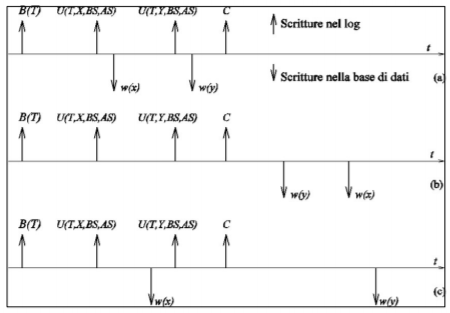
\includegraphics{images/136.PNG}
\end{center}
\begin{itemize}
	\item \textbf{Modalità immediata}: il database contiene valori $AS$ provenienti da transazioni uncommited. In caso di guasto devo fare undo, non ho bisogno di fare redo.
	\item \textbf{Modalità differita}: il database non contiene valori $AS$ provenienti da transazioni uncommited. In caso di aborto non bisogna fare niente. L'undo è superfluo, poichè non si hanno operazioni di scrittura prima del commit. In caso di guasto rieseguo le operazioni.
	\item \textbf{Modalità mista}: la scrittura avviene in modalità sia immediata che differita, ricorrendo se necessario sia all'undo che al redo.
\end{itemize}
La modalità differita non è molto utilizzata pur permettendo una procedura di recovery più semplice ed efficiente: questo perchè il gestore del buffer non è libero di decidere quando scrivere in memoria secondaria. Risulta preferibile una gestione ordinaria più efficiente rispetto a una più semplice dei guasti, considerando la rarità di questi.
\paragraph{In conclusione}
\begin{itemize}
	\item La scrittura nella base di dati può avvenire in qualunque momento, anche prima del commit
	\item La scrittura sul log è effettuata prima della scrittura nella base di dati
	\item Il commit si considera effettuato quando il corrispondente record di log è scritto. Prima di questa scrittura il guasto causa l'undo; dopo il guasto causa il redo.
\end{itemize}
\subsection{Rollback di una transazione} Quando una transazione deve essere cancellata tutte le operazioni tra il begin della transazione e l'abort devono essere disfatte. Sarà scritto un record di abort nel log. Distinguiamo i seguenti tipi di guasti
\begin{itemize}
	\item \textbf{Guasti soft}: errori di programma, crash di sistema, caduta di tensione. Si perde la memoria centrale ma non quella secondaria (la base di dati e il log).\\
	\small In questo caso avremo un \emph{warm restart}, cioè una \textbf{ripresa a caldo} \normalsize
	\item \textbf{Guasti hard}: si perde anche la memoria secondaria, cioè parte della base dei dati. Ovviamente non si perde la memoria stabile contenente i log.\\
	\small In questo caso avremo un \emph{cold restart}, cioè una \textbf{ripresa a freddo} \normalsize
\end{itemize}
La perdita dei \emph{log} o dei \emph{dump} è considerato un evento catastrofico, uno dei più improbabili, e quindi non è definita alcuna strategia di recupero.
\paragraph{Cosa fa il gestore in caso di guasti?} Il modello adottato è quello \emph{fail-stop}
\begin{itemize}
	\item Si forza l'arresto completo delle transazioni
	\item Il sistema operativo viene riavviato
	\item \textbf{Viene avviata una procedura di restart} (che sarà a caldo o a freddo)
	\item Al termine del restart il buffer è vuoto, ma le transazioni possono ripartire.
\end{itemize}
Considero la seguente classificazione di transazioni nel processo di restart:
\begin{itemize}
	\item Transazioni completate (i dati sono in memoria e non dobbiamo fare niente)
	\item Transazioni attive ma con commit (da rifare, \emph{redo})
	\item Transazioni attive ma senza commit (da annullare, \emph{undo})
\end{itemize}
\subsubsection{Processo di restart a caldo}
\paragraph{Fasi}
\begin{enumerate}
	\item Trovare l'ultimo checkpoint (ripercorrendo il log a ritroso)
	\item Costruire gli insiemi UNDO e REDO, cioè individuare le transazione da disfare e quelle da rifare. 
	\begin{itemize}
		\item Inizializzo UNDO con le transazioni attive al checkpoint. REDO inizialmente è vuoto.
		\item Aggiungo all'insieme di UNDO tutte le transazioni che presentano un record di begin e sposto in REDO tutti gli identificativi delle transazioni in cui è presente record di commit.
		\item Al termine i due insiemi conterranno, appunto, gli identificativi delle transazioni da disfare e di quelle da rifare
	\end{itemize}
	\item Ripercorrere il log all'indietro fino alla più vecchia azione delle transazioni in UNDO e REDO, disfacendo tutte le azioni delle transazioni in UNDO.
	\item Ripercorrere il log in avanti, rifacendo tutte le azioni delle transazioni in REDO.
\end{enumerate}
\paragraph{Esempio 1} Considerando il seguente log di un sistema di gestione di basi di dati, illustrare dettagliatamente i passi da compiere per effettuare la ripresa a caldo.\\

\noindent Dump, B(T1), B(T2), I(T1,O1,A1), D(T2,O2,B2), B(T3), B(T4), U(T3,O3,B3,A3), C(T2), CK($\boxed{\dots}$), U(T1,O4,B4,A4), A(T3), B(T5), D(T4,O5,B5), C(T1), C(T4), I(T5,O6,A6), GUASTO

\begin{itemize}
	\item Le transazioni attive (cioè quelle che scrivo nel checkpoint) sono T1,T3 e T4.
	\item T2 è già terminata, quindi ci interessa poco
	\item Realizzo i due insiemi di \emph{UNDO} e \emph{REDO}
	\begin{center}
		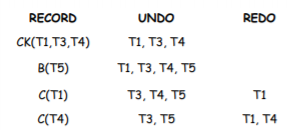
\includegraphics{images/137.PNG}
	\end{center}
	\item Le transazioni da disfare sono T3 e T5, mentre quelle da rifare sono T1 e T4. Riempo la tabella delle UNDO partendo dal fondo e considero le operazioni di T3 e T5.
	\begin{center}
		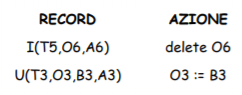
\includegraphics{images/138.PNG}
	\end{center}
	\item Si riempe la tabella delle REDO partendo dall'inizio e considerando le operazioni di T1 e T4
	\begin{center}
		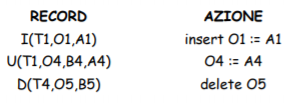
\includegraphics{images/139.PNG}
	\end{center}
\end{itemize}
\paragraph{Domanda} Le transazione attive da inserire nel checkpoint si possono fissare: 
\begin{itemize}
	\item Rifiutando nuovi commit
	\item Rifiutando nuove transazioni e aspettando la conclusione di quelle già iniziate
\end{itemize}
Quale sarà la differenza nella gestione delle riprese a caldo? 
\begin{itemize}
	\item Nel primo caso si attua la strategia già vista
	\item Nel secondo caso il checkpoint non conterrà nessuna transazione poichè non si hanno transazioni attive. Nella ripresa a caldo mi limito a rieseguire tutte le operazioni che seguono il record di checkpoint. 
	\begin{itemize}
		\item Una conseguenza è il degrado delle prestazioni poichè la base di dati viene fermata ogni volta che si deve eseguire un checkpoint. 
		\item Inoltre questi errori sono rari.
		\item Segue che la prima soluzione è più conveniente: è improduttivo semplificare la gestione di questi errori (rari) se ciò comporta una gestione più complicata delle situazioni ordinarie.
	\end{itemize}
\end{itemize}
\paragraph{Transazioni abortite} Le operazioni derivanti dal rollback di una transazione possono essere inserite nell'insieme UNDO e fatte al momento del recovery, oppure essere eseguite al momento dell'abort venendo inserite nell'insieme di redo al momento del recovery da un guasto.

\subsubsection{Ripresa a freddo}
\paragraph{Fasi}
\begin{itemize}
	\item Ci si riporta al record di dump più recente nel log e si ripristina la parte di dati deteriorata
	\item Si eseguono le operazioni registrate sul log nella parte deteriorata fino all'istante del guasto
	\item Si esegue una ripresa a caldo
\end{itemize}
\paragraph{Esempio 2} Riprendio lo stesso log di prima. Considerando il seguente log di un sistema di gestione di basi di dati, illustrare dettagliatamente i passi da compiere per effettuare la ripresa a freddo dopo un guasto di dispositivo che interessa gli oggetti O1, O2, O3.

\begin{itemize}
	\item Insert O1 = A1
	\item Delete(O2)
	\item O3=A3
	\item Commit(T2)
	\item Abort(T3)
	\item Commit(T1)
	\item Commit(T4)
	\item Ripresa a caldo
\end{itemize}